\section{Markt}
\subsection{Einleitung}
Im folgenden Kapitel soll ein grober Überblick und eine Einleitung zum IT-Consulting Markt gegeben werden. 
Ziel einer solchen Recherche sowohl Informationen zu sammeln, die strategische Möglichkeiten für Expansion, Kooperation oder Offshoring (Outsourcing ins Ausland)  aufzeigen, 
als auch die Wettbewerbssituation besser einzuschätzen, um daraus Handlungsalternativen abzuleiten. 
In zahlreichen Studien tauchen in diesem Zusammenhang häufig sehr weitgefasste Begriffe auf wie „technology industry“ oder "IT-service-market" auf. 
Die Grenzen der Bandbreite der darin enthaltenen Beratungsleistungen sind darum besonders unscharf. Eine Differenzierung ist aufgrund der Komplexität der Zusammensetzung des Dienstleistungsspektrums daher nur im groben Umfang möglich.
Deswegen wurde darauf geachtet, dass die erfassten Unternehmen einen Mindestanteil  für ausschließlich beratende Tätigkeiten von mindestens 40\%  aufweisen, um in eine IT-Consulting äquivalente Kategorie zu fallen.
Es gibt zahlreiche Schlüsselfaktoren, die für die Einschätzung des Marktes in den jeweiligen Ländern bzw. Kontinenten aufschlussreich sind. 
Allerdings ist eine Erhebung sehr zeitaufwändig oder/und teuer. Es gibt zahlreiche Marktstudien von großen Marktforschungsunternehmen, wie z.B. Gartner, die man ab ca. 1000 €  erwerben kann, die aber nur Teilaspekte abdecken. 
Es gibt kaum kostenfreie umfassendere Studien zu dem gesamten Thema, dafür jedoch zahlreiche kostenpflichtige Studien zu hohen Preisen. Es lässt sich daher vermuten, dass es zumindest aufgrund des niedrigen Angebots an kostenlosen Studien, eine moderate Nachfrage nach kostenfreien Marktinformationen im Bereich des IT-Consulting gibt. Ob die kostenpflichtigen Studien den Informationsbedarf abdecken würden, gilt es daher zu prüfen und zu erwägen, ob eine Investition darin lohnt.

 Ziel des Kapitels ist es, sich dem  Thema zuerst theoretisch anzunähern und die Schlüsselfaktoren zu überlegen und deren konkrete Größen zu ermitteln. Anschließend erfolgt eine Untersuchung einzelner Teilaspekte.

\subsection{Teilaspekte}
Nachfolgend soll zuerst einmal begründet werden, welche Teilaspekte für eine Marktrecherche im IT-Consulting für eine Studie als besonders relevant erachtet werden.
Ein Großteil der Arbeit liegt deswegen vor allem in der Ermittlung des Informationsbedarfes um zu entscheiden, welche Kenngrößen als Faktoren überhaupt relevant sind.
Sichere Prognosen können daraus nicht in jedem Fall resultieren, da die gewählten Teilaspekte und deren Faktoren auf vernünftige Schätzungen beruhen und die Marktaspekte dynamische Faktoren eines komplexen und chaotischen System sind. Es lassen sich auf dieser Basis  jedoch vernünftige Schlussfolgerungen ziehen, die es wiederum zu verifizieren gilt. Statistische Verfahren bieten hier eine Möglichkeit, um zumindest eine hohe Wahrscheinlichkeit zu erreichen. 
Wie derart vage Informationen in eine Entscheidung einbezogen werden, bleibt außen vor. Es gibt jedoch zahlreiche Verfahren in der Entscheidungstheorie, welche unsichere Umstände in Managemententscheidungen einbeziehen. Letztendlich kommt es auf den Anwendungszweck der Information an, ob diese für eine Entscheidung relevant ist.
 
\subsubsection{Gewinn- und Umsatzzahlen von Großunternehmen weltweit/Länder spezifisch}
Diese Daten sind gut zugänglich und liefern eine grobe Richtzahl über Umsatz und Erfolg in der Branche in dem jeweiligen Land. Hauptziel ist es eine Nachfrage aus den Kennziffern abzuleiten. So lassen sich anhand des Vergleiches der Umsatzzahlen und Gewinne der gleichen Unternehmen in verschiedenen Ländern Rückschlüsse auf mögliche Ursachen ziehen.
 Es muss hierbei jedoch berücksichtigt werden, ob die Großunternehmen nur Großprojekte übernehmen oder auch kleine bis mittlere Projekte. Sollte der hohe Umsatz maßgeblich durch Großprojekte generiert werden, muss dies nicht gleichermaßen kleine und mittlere Unternehmen gelten.
Des Weiteren dienen diese Daten dazu, die erfolgreichsten Unternehmen zu ermitteln, um diese anschließend zu beobachten und deren Wettbewerbsvorteile zu erkennen. Dieses Wissen liefert Hinweise auf Indikatoren, die zu dem Erfolg eines Unternehmens in dem jeweiligen Land beigetragen haben.
 So kann ein Unternehmen, welches z.B. auf SAP spezialisiert ist, zwar in Brasilien erfolgreich sein, jedoch in China trotz guter Marktlage nicht. Ursachen liegen in diesem Fall nicht im Markt, sondern z.B. in der strategischen Ausrichtung der IT in chinesischen Unternehmen (z.B. Kostendruck, kurzsichtige Denkweise) oder weil es sehr starke Konkurrenten gibt.
Signifikante Unterschieden bieten Potential um Vermutungen aufzustellen und diese weiter zu untersuchen oder um allgemeine Unterschiede im Erfolgspotential zwischen Ländern abzuleiten. 

\subsubsection{IT-Consulting Gesamtumsatz und Marktwachstum je Land}
Diese Kennzahlen liefern wichtige Hinweise, wie sich die Branche weiter entwickeln wird und wie sehr sie schon entwickelt ist. 
Diese Daten dienen dazu um Rückschlüsse auf die Nachfrage von IT-Consulting-Leistungen zu ziehen. 
Dazu werden natürlich noch eine Reihe weiterer Daten benötigt, wie Gesamtmarktvolumen und Gesamtwirtschaftswachstum, um die Kennzahlen ins Verhältnis zu setzen.
 Außerdem muss darauf geachtet werden, welche Umstände die Kennzahlen verfälschen wie z.B. die Ländergröße, wodurch eher ein höherer Umsatz pro Land entsteht. 
 Es werden deswegen weitere Kennzahlen wie z.B. Fläche des Landes oder Einwohnerzahlen benötigt, um diese Faktoren ordnungsgemäß bewerten zu können.
Der IT-Consulting-Umsatz und das Wachstum je Land ist im Verhältnis zu anderen Kenngrößen durchaus im vertretbaren Umfang anhand von öffentlichen Studien erfassbar.  
Daher sollen diese Größen einzeln nach Ländern aufgelistet und erläutert werden. 
 Dabei ist zu berücksichtigen, dass auf die daraus resultierenden Anteile und Kennzahlen, dem Anspruch auf Korrektheit nicht gerecht werden kann. 
 Hierfür müssen diese Kennziffern noch mehrfach überprüft und Einflüsse die zur Verwässerung der Faktoren führen, herausgerechnet werden, um eine möglichst genaue Einschätzung zum Marktanteil und dem Wachstum zu treffen. Da dies jedoch den Rahmen der Arbeit sprengen würde, wird zunächst eine vereinfachte Betrachtung vorgenommen. Diese kann bei Bedarf als Ausgangsbasis  verwendet werden, um eine korrigierte Aussage zu treffen. 
 Für einen generellen Überblick und eine grobe Quantifizierung sind sie jedoch durchaus brauchbar. So können auf Basis dieser weitere Vermutungen angestellt und entsprechende Recherchen unternommen werden.
Es wurde sich dazu entschieden diesen Teilaspekt für die Recherche auszuwählen. (siehe  \ref{subsubsec:Gesamtumsatz} \nameref{subsubsec:Gesamtumsatz} auf Seite \pageref{subsubsec:Gesamtumsatz})



 \subsubsection{Firmengrößen im IT-Consulting}
Ein wichtiger Einflussfaktor um die Konkurrenzsituation festzustellen, ist die Beschaffenheit des Marktes nach Unternehmensgrößen.
 Es stellt sich die Frage, ob eher Großkonzerne, mittelständische und kleine  Unternehmen oder gar interne Mitarbeiter für die strategische und ganzheitliche Gestaltung der IT beauftragt werden.
Es kann zum einen die durchschnittliche Firmengröße eines IT-Consulting Unternehmens herangezogen werden  und zum anderen die prozentualen Anteile der einzelnen Sektoren.  Es gibt Länder, die eher einen breiten Mittelstand haben oder eher von Großkonzernen dominiert werden. 
Ziel einer solchen Analyse ist es, Häufungen oder Bedarfe in einzelnen Sektoren festzustellen. 
Beispielsweise ein mittelständisches Unternehmen könnte, wenn es nur einen geringen Anteil kleiner und mittelständischer Unternehmen gibt, von einem erhöhten Bedarf in der IT-Beratung mit kleiner bis mittlerer Projektgröße profitieren, in so fern die Großunternehmen nur an großen Projekten interessiert sind.

Die Möglichkeiten zur Ermittlung der Marktbeschaffenheit bestehen aus  folgenden Schritten:
\begin{itemize}
\item Statistische Stichproben / Befragungen zur Ermittlung der Anteile
\item Analyse Dienstleistungsangebote der IT-Consulting-Unternehmen in dem jeweiligen Sektor 
\item Berechnung der Marktanteile der größten Unternehmen und Bewertung des Restwertes zum Vergleich mit der Stichprobe
\item Beschaffung von Studien oder Beauftragung eines Marktforschungsunternehmen, falls die Stichproben nicht ausreichen
\end{itemize}
Die resultierenden Informationen zur Beschaffenheit geben wertvolle Hinweise über das Angebot in der Branche des IT-Consulting. 
So können von diesem Wissensstandpunkt aus die konkreten Angebote analysiert werden und ggf. Chancen abgeleitet werden. 
Beispielsweise können große Unternehmen aufgrund ihrer Kosteneffizienz möglicherweise bessere Qualität anbieten als ein breiter Mittelstand, gleichzeitig die Nachfrage nach mittelständischen Unternehmen aufgrund günstigerer Preise höher sein. 
Eine tiefgehende Analyse ist jedoch sehr komplex und würde Stoff für eine eigenständige Studie liefern und soll deswegen kein weiterer Gegenstand sein.

 \subsubsection{Politik / Rechtslage}
Die politische und rechtliche Lage ist ein wichtiger Faktor für die Wahl eines Standortes oder die Zusammenarbeit mit einem Land. Gleichzeitig ist es ein Teilaspekt, der die Entwicklung der Branche beeinflusst.
Besonderen Einfluss haben die folgenden Faktoren auf die IT-Consulting Branche:
\begin{itemize} 
\item {generelle staatliche Subventionen / Investitionen in die IT}

 Staatliche Förderprogramme und Subventionen für IT-Entwicklungen stellen eine wichtige Finanzierungsmethode für Entwicklungsprojekte oder Unternehmen, deren Existenz bedroht ist, dar. Diese Subventionen bestehen beispielsweise aus zinsgünstigen Darlehen oder Fördermitteln, die nicht zurückgezahlt werden müssen. Die unterschiedlichen Arten von Fördermitteln müssen daher klassifiziert und entsprechend eingeordnet werden
 Solche finanziellen Unterstützungen treiben natürlich die Forschung und den allgemeinen Wissenstransfer voran. Insbesondere das IT-Consulting ist eine reine Wissensbranche. Wenn die IT-Entwicklung von Unternehmen profitiert, profitiert auch das IT-Consulting von den neuen Erkenntnissen. 
 Staatliche Finanzierungsformen können als Anreiz für Unternehmensgründungen dienen und damit die Innovativität der IT-Landschaft fördern. Neue Technologien und Erkenntnisse führen zu neuen Handlungsalternativen. Das Wachstum in der IT-Branche erhöht wiederum die Komplexität von Entscheidungsprozessen und Nachfrage nach Beratungsleistungen.
Ein Wissen über Staatssubventionen kann daher hilfreich sein, um das Entwicklungspotential und das Maß an finanzieller Stabilität für Unternehmens-Neugründungen, welche durch Förderprogramme erhöht werden kann, einzuschätzen.
 \\
\item  {Handelsrecht / Arbeitsrecht}

 Das Vertrags-und Arbeitsrecht hat Einfluss auf das Outsourcing oder die Kooperationen mit einem ausländischen Unternehmen. 
 So sind in jedem Land bestimmte Handels und Arbeitsgesetze zu beachten, die eine reibungslose Unternehmens-Kooperation oder ein rechtmäßiges Arbeitsverhältnis gewährleisten. 
Für das Unternehmen steht vor allem die Frage nach der Haftung und Behandlung von Mängeln im Vordergrund. 
Eine Einordnung nach Risiken und Chancen ist hier folglich notwendig, um das Land zu beurteilen. 
 \\
\item {Steuerrecht}

 Das Steuerrecht ist vor allem für die Standortwahl ausschlaggebend. 
 So sind möglicherweise bestimmte Besteuerungsvorschriften mit in die strategische Standortauswahl einzubeziehen. So gilt es abzuwägen, ob die Gewinnerwartungen nach Steuern höher sind, als in einem anderen Land. Zahlreiche Unternehmen suchen sich Ihren Hauptsitz daher nach den für Sie günstigen Steuervorteilen aus.
 Allerdings gilt es verschiedene Punkte zu analysieren wie:
 - Höhe der Mehrwertsteuer
 - Legalität bei Dienstleistungsvertrieb und Aufenthalt in einem anderen Land
 - Höhe der Einkommensteuern
 - Höhe der Gewerbesteuer/Grundsteuer
 - Spezielle Sonderregelungen
  \\
\item {Datenschutz/Urheberrecht}

  Der Datenschutz ist ausschlaggebend für den Austausch von sensiblen Unternehmensdaten. 
  Die Gefahr von Produktpiraterie oder der Weitergabe von sensiblen Daten kann ein Risiko für Kooperation mit Partnern, Expansion oder dem Outsourcing sein. Ursachen liegen hier in zu schwachen oder gar nicht vorhandenen Gesetzen für das Urheberrecht oder dem Datenschutz.
  
  \end{itemize}
\subsubsection{Lohnniveau}
\subsubsection{Fachkräftemangel / Bedarf}
\subsection{Analyse ausgewählter Teilaspekte}
\subsubsection{IT-Consulting Gesamtumsatz und Marktwachstum je Land}
\label{subsubsec:Gesamtumsatz}

\begin{itemize} 
\item {Global}

Insgesamt wurden 2010 laut Gartner 574,94 Milliarden Euro weltweit in der IT-Consulting-Branche umgesetzt. \cite{itConsultingGlobal} Das durchschnittliche globale jährliche Wachstum beträgt 2,6\% zwischen 2007 und 2011.\cite{globalGartner}

\begin{figure}
  \centering
  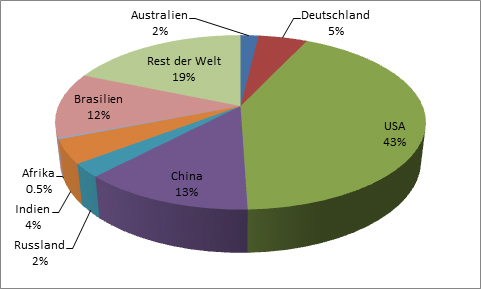
\includegraphics[width=0.8\textwidth]{images/global_revenue_share.jpg} 
  \caption{Anteile am IT-Consulting Weltmarkt} \label{fig:weltmarkt} 
\end{figure}


\item {Deutschland}

Das Wachstum des deutschen IT-Consulting ist mit 8,4\% sehr hoch im Verhältnis des Wirtschaftswachstums von 3\% in 2011.\cite{statGer2} Dabei haben die Top 25 IT-Consulting- Unternehmen sogar noch ein größeres Wachstum mit Spitzen bis zu 10\%. \cite[6]{topITB} Dies sind durchaus überdurchschnittliche Wachstumsraten, welche international mit aufsteigenden Ökonomien wie Indien, Russland oder China sehr gut mithalten können.  (siehe  \ref{table:umsaetze} \nameref{table:umsaetze} auf Seite \pageref{table:umsaetze}) Der Gesamtumsatz des IT-Consulting beträgt 29,4 Milliarden Euro.  Das sind 1,12 Prozent des gesamten bereinigten Bruttoeinlandproduktes. \cite{statGer} Um die Dichte des IT-Consulting-Marktes einschätzen zu können macht es Sinn den Gesamtumsatz auf die Ländergröße zu beziehen. 
Deutschland erzielt 8,24 Milliarden Euro pro 100000 km² ab. Dies ist im Vergleich mit den anderen Ländern eine enorm hohe Dichte und bietet dadurch eher Wegersparnisse und Kommunikationsvorteile, die sich strategisch günstig auswirken können. 

\item {USA}

Die USA zweifellos einen gigantischen Marktanteil an IT-Services. Mit 244 Milliarden Euro, was 43\% des weltweiten IT-Service Markt einnimmt, ist es mit Abstand das umsatzstärkste Land der Welt im Bereich IT-Services. \cite{ibisUSA} Das Wachstum stagniert allerdings mit 2,2\%. Im Verhältnis zum Wachstum des bereinigten Bruttoninlandsproduktes von 1,8\% wächst es nur wenig mehr. \cite{statUSA} Die Dichte des IT-Consulting-Marktes beträgt 2,48 Milliarden Euro pro 100000 km². Im Verhältnis zu anderen Ländern wie z.B. Indien oder Russland ist dies eine sehr hohe Dichte, nur Deutschland schneidet noch deutlich besser ab.

Ein Großteil der Umsätze in den USA entsteht unter anderem dadurch, dass Wertschöpfung durch IT-Services, die im Ausland durch Offshoring entstehen, hinzugerechnet werden. Diese Offshoring-Länder sind daher einer der Schlüsselfaktoren für die hohen Umsätze in den USA. 

\item {China}

China hat mit 72,6 Milliarden Euro den zweitgrößten Marktanteil der Welt. Es hat zwar noch weniger als ein Drittel gegenüber den USA, jedoch verzeichnet es mit 6,8\% in 2011 überdurchschnittliche Wachstumsraten im Bereich IT-Services und hat damit das dreifache Wachstum des Konkurrenten USA.  Im Verhältnis zum Wachstum des Bruttoinlandsproduktes mit 9,2\% in 2011 ist das Wachstum jedoch verhältnismäßig wenig. Dieses Verhältnis deutet stark daraufhin, dass die strategische Ausrichtung der IT und deren Prozessen noch nicht gleichermaßen Beachtung geschenkt wird, wie anderen Dienstleistungen und Produkten. Mögliche Ursachen könnten Fachkräftemängel oder Kostendruck sein. Es gilt daher weiter zu untersuchen, welche Ursachen das verhältnismäßig schwächere Wachstum hat. 
Die Wachstumsraten im Bereich IT-Services sind in alle Ländern über dem des BIP. Warum dies in China so weit nach unten abweicht ist, gilt es daher weiterhin zu untersuchen und dafür Ursachen zu finden.
Die Dichte ist im Verhältnis zu Deutschland oder den USA auch deutlich schwächer. Hier schneidet China mit einer IT-Service-Dichte von 0,74 Milliarden pro 100000 km² ab. Da China sehr weitläufig und nicht vollständig industrialisiert ist, ist diese Größe wenig aussagekräftig und es besteht weiterer Untersuchungsbedarf, ob diese Größe wirklich auf einen schwächer entwickelten IT-Consulting-Markt hindeutet oder anderen demografischen Umständen geschuldet ist. \cite{ibisChina}

\item {Russland}

Der russische Markt im Bereich IT-Services ist mit 14,3 Milliarden recht klein wenn man es auf die Größe des Landes bezieht. Es gibt vor allem viel System- und hardwarenahe Entwicklung. Dienstleistungen im IT-Sektor wachsen jedoch in zunehmenden Maße und konnten 2011 15,3\% Branchen-Wachstum erreichen. Dies ist sowohl im Vergleich zum internationalen Markt als auch im Verhältnis zum Wachstum des Bruttoinlandsproduktes mit 4,3 \% in 2011 weit überdurchschnittlich. \cite{statRus2} Aufgrund der relativ kostengünstigen Entwicklungskosten für Software, insbesondere hardwarenahe Entwicklung und Systemengineering wird Russland vor allem in Europa zunehmend als „Offshoring Land“ attraktiv. (Wirtschaftsinformatik und Management 12/2013, Offshoring Land Russland)
Die Dichte des IT-Consulting fällt mit 84 Millionen Euro pro 100 000 km² sehr klein aus. Dabei ist zu berücksichtigen, dass ein Großteil von Russland gar nicht oder nur schwach bewirtschaftet ist. \cite{statRus}


\item {Afrika}

Afrika hat einen sehr niedrigen Anteil am Markt mit 1,4 Milliarden. \cite{statAfr} Statistiken zum Wachstum konnten leider nicht gefunden werden. Die großen Technologie-Beratungs-Konzerne haben sich in verschiedenen Teilen Afrika als Beratungen etabliert, die auch den IT-Consulting Markt abdecken. Der Trend geht jedoch laut Experten immer mehr dahin, dass neue inländische IT-Service-Provider auf dem Markt konkurrieren und die US-Konzerne ablösen. Afrika hat 2011 mit 5\% ein durchaus gutes Wirtschaftswachstum zu verzeichnen, kann aber nicht mit anderen aufstrebenden Ökonomien mithalten, insbesondere nicht im IT-Umfeld. \cite{statAfr2}
Ursachen liegen hier nicht zuletzt in der Stromversorgung. Denn 80\% der Dörfer in Afrika sind immer noch ohne Stromversorgung, weil Energieanbietern die Vernetzung der Dörfer zu teuer ist.  \cite{dieZeit}
Die Situation des Marktes im gesamten Kontinent ist jedoch sehr vielschichtig. Eine Analyse des Marktes in sehr komplex, da in Afrika sehr viele demografische und infrastrukturelle Umbrüche stattfinden. Daher ist hier eine Betrachtung der Umsätze wenig aussagekräftig für eine klare Einschätzung. 
Um eine besser Bewertung zu ermöglichen, ist eine Unterteilung von Afrika notwendig. Des weiteren sind die Kennzahlen, aufgrund der hohen Marktdynamik, aus nur einem Jahr nicht ausreichend aussagekräftig. Deswegen ist es sinnvoll die Umsätze und Wachstumsraten, noch ein einem größeren Zeitraum zu betrachten.
Es besteht daher hier weiterer Forschungsbedarf, um die Kennzahlen in einem differenzierteren Kontext zu stellen.
Die Werte eignen sich daher mehr für den Vergleich der IST-Situation mit anderen Ländern.


\item {Brasilien}

Brasilien hat im Jahre 2011 mit einem Branchenumsatz von 69,6 Milliarden, den drittgrößten Anteil am globalen IT-Consulting Markt erzielt. Das Wachstum über die Jahre von 2008-2011 beträgt 61\%. \cite{statBras2} Trotz seiner flächenmäßigen Größe weist es mit 0,82 Milliarden pro 100 000 km eine verhältnismäßig hohe Dichte auf. Das Wachstum in 2011 in der IT-Services-Branche beträgt hier 4,9\% und ist damit weitaus höher als das Gesamtwirtschaftswachstum mit 2,7\%. Dabei beträgt der Anteil am Bruttoinlandsprodukt allein 4,5\%. Dies zeigt welchen großen Stellenwert der Markt für IT-Services in Brasilien einnimmt. Experten prognostizieren weiterhin einen rasanten Anstieg des Wachstums, insbesondere im Bereich BPO, welche laut Schätzungen 85\% am Gesamtmarktanteil einnimmt.\cite{statBras}

\item {Zusammenfassung}

Alle Werte beziehen sich auf die Jahre von 2011 bis 2012. Die entsprechenden Quellen sind in den Länderabschnitten zu finden.


\begin{table}

\caption{Übersicht Umsatz und Umsatzwachstum von IT-Services im Verhältnis zum BIP  (2010)}
\begin{tabular}{|p{2.6cm}|p{1.5cm}|p{2cm}|p{1.5cm}|p{1.5cm}|p{1.7cm}|}
 \hline
  \textbf{Land} & \textbf{Umsatz in Mrd. €} & \textbf{IT-Consulting Wachstum} & \textbf{BIP Wachstum} & \textbf{Welt-Markt-Anteil} & \textbf{Umsatz-Dichte in Mrd. € pro 100 000 km²} \\
  \hline
    
    1. USA  & 244,33  &2,2\%  & 1,8\% & 43\% & 2,48  \\
    2. China & 72,50 & 6,8\%  & 9,2\% & 13\% & 0,74 \\
    3. Brasilien & 69,60 & 4,9\%  & 2,7\% & 12\% & 0,817 \\
    4. Deutschland & 29,4 & 8,5\%  & 3\% & 5\% & 8,24 \\
    5. Indien & 25,45  & 11.2\%  & 7.9\% & 4\% & 0,77  \\
    6. Russland & 14,3  & 15.4\%  & 4,3\% & 2\% & 0,084  \\
    7. Afrika & 1.4  & n/a  & 5\% & 0.5\% & 0,0046 \\
 \hline
\end{tabular}
\label{table:umsaetze} 
\end{table}

\end{itemize}


